\documentclass[a4paper,12pt]{report}

\usepackage[utf8]{inputenc}
\usepackage{amsmath}
\usepackage{fontspec}
\usepackage{float}
\usepackage{enumitem}
\usepackage{graphicx}
\usepackage{wrapfig}
\usepackage{setspace}
\usepackage[titletoc]{appendix}
\usepackage{pdfpages} 
\usepackage{cite}
\usepackage{url}
\usepackage{listings}
\usepackage{color}

\definecolor{codegreen}{rgb}{0,0.6,0}
\definecolor{codegray}{rgb}{0.5,0.5,0.5}
\definecolor{codepurple}{rgb}{0.58,0,0.82}

\lstdefinestyle{mystyle}{
	backgroundcolor=\color{white},   
	commentstyle=\color{codegreen},
	keywordstyle=\color{blue},
	numberstyle=\tiny\color{codegray},
	stringstyle=\color{codepurple},
	basicstyle=\footnotesize,
	breakatwhitespace=false,         
	breaklines=true,                 
	captionpos=b,                    
	keepspaces=true,                 
	numbers=left,                    
	numbersep=5pt,                  
	showspaces=false,                
	showstringspaces=false,
	showtabs=false,                  
	tabsize=2
}

\lstset{style=mystyle}

\setlength{\parindent}{0em}
\setlength{\parskip}{0.5em}

\setmainfont[
BoldFont=arialbd.ttf,
ItalicFont=ariali.ttf,
BoldItalicFont=arialbi.ttf
]{arial.ttf}

\author{Arundathi Shaji Shanthini}


\renewcommand{\bibname}{References}

%\setlength{\voffset}{-0.75in}

\begin{document}
%%%%%%%%%%%COVERSHEET%%%%%%%%%%%%%%%%%
\begin{titlepage}
    \setlength{\voffset}{-1.8in}
    \noindent \noindent \makebox[\textwidth]{
\includegraphics[width=1.55\textwidth]{images/Coversheet_Header_black_with_text.png}}
    
    \vspace{30mm}

    \begin{center}
        {\LARGE \textbf{BEng Project}}\\
        \vspace{4mm}
        {\Huge \textbf{Final Report}}
    \end{center}
    
    \vspace{10mm}
    
    \begin{center}
    \begin{spacing}{1.8}
    {\LARGE
   Dynamic Modelling of a Continuum Robotic Snake-arm and its Performance Evaluation by Analysing Robustness}
    \end{spacing}
    \end{center}
    
   \vspace{5mm}
    
     \begin{tabular}{ll}
        \textbf{Student Name:}  & \hspace{4mm} Arundathi Shaji Shanthini \\
       \textbf{Contact e-mail:} & \hspace{4mm} arundathi.shanthini.16@ucl.ac.uk \\
        \textbf{Student number:} & \hspace{4mm} 16018351 \\ \\ 
        \textbf{Project Supervisor:}  & \hspace{4mm} Prof. Sarah Spurgeon \\
        \textbf{Contact e-mail:}  & \hspace{4mm} s.spurgeon@ucl.ac.uk \\
         \textbf{Department:} & \hspace{4mm} Department of Electronic and Electrical Engineering\\ \\ 
          \textbf{Submission Date:} & \hspace{4mm} 13\textsuperscript{th} of December 2019
    \end{tabular}
\end{titlepage}
%%%%%%%%%%%%%%%%%%%%%%%%%%%%%%%%%%%%%%

\pagebreak

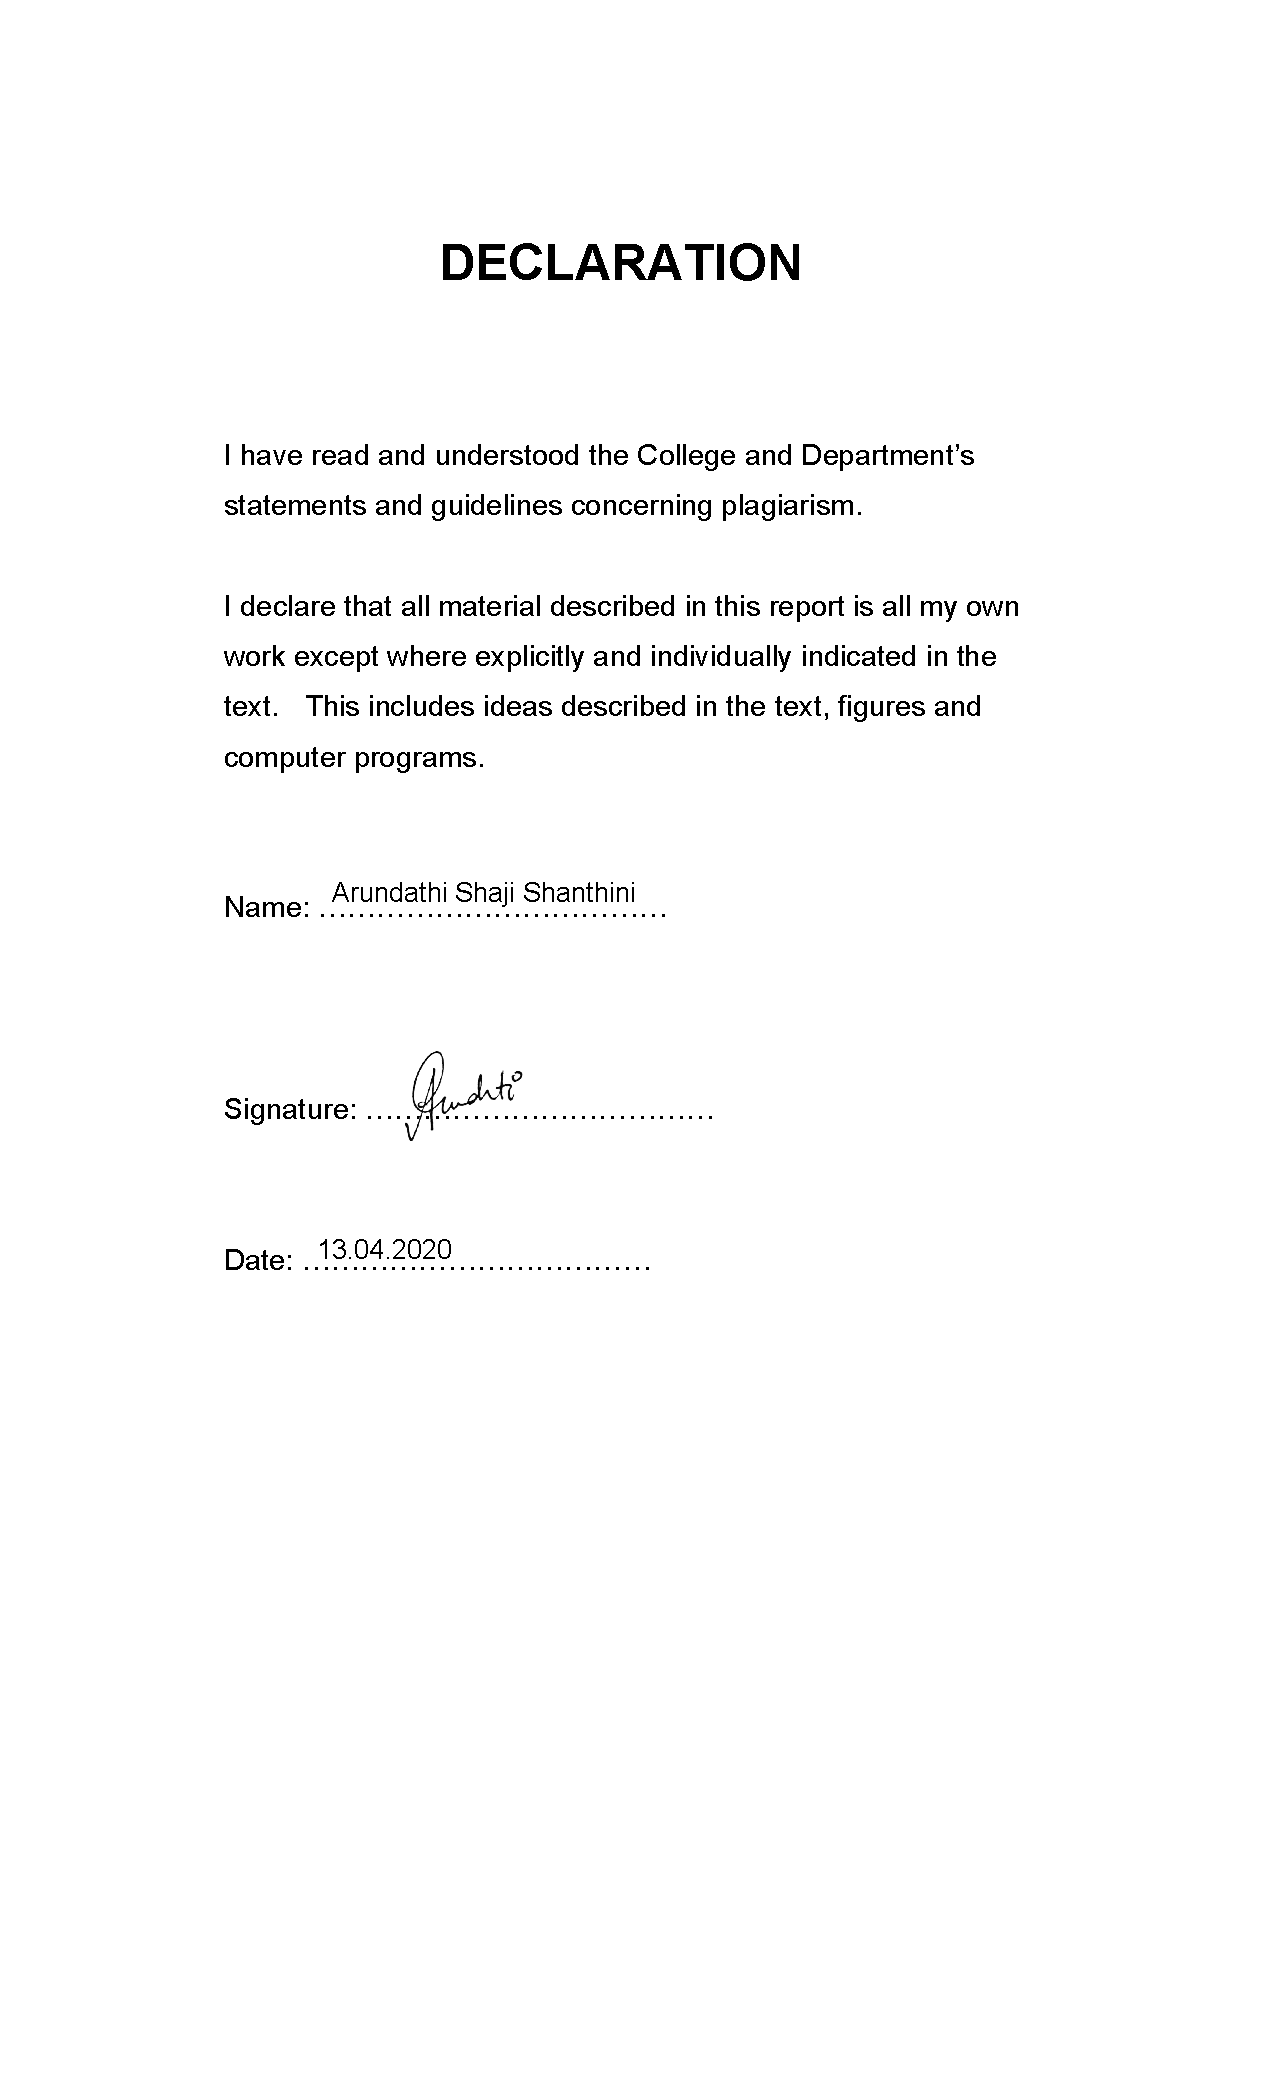
\includepdf[page=-]{files/Declaration}

\tableofcontents

\pagebreak

%%%%%%%%%%% ABSTRACT %%%%%%%%%%%%%%%%%
\begin{abstract}
    
    
\end{abstract}
%%%%%%%%%%%%%%%%%%%%%%%%%%%%%%%%%%%%%%

%%%%%%%%%%% INTRODUCTION %%%%%%%%%%%%%%%%%
\chapter{Introduction}
\section{Project Description and Motivations}

\section{Literature Review}

\section{Aims and Objectives}


%%%%%%%%%%%%%%%%%%%%%%%%%%%%%%%%%%%%%%

%%%%%%%%%%% MATHEMATICAL MODELLING %%%%%%%%%%%%%%%%%
\chapter{Mathematical Modelling}

\section{Understanding the system}


\section{Kinematic Modelling}


\subsection{Cable Length - Joint Angle Kinematics}

\subsection{Joint Angle - End Effector Pose Kinematics}

\section{Dynamic Modelling}



%%%%%%%%%%%%%%%%%%%%%%%%%%%%%%%%%%%%%%

%%%%%%%%%%% MATHEMATICAL MODELLING %%%%%%%%%%%%%%%%%
\chapter{Implementation and Simulation}


\section{Implementation on Simulink}

\subsection{Motor Angle of Rotation - Cable Length Kinematics}

\subsection{Cable Length - Joint Angle Kinematics}


\subsection{Joint Angle - End Effector Pose Kinematics}



%%%%%%%%%%%%%%%%%%%%%%%%%%%%%%%%%%%%%%

\chapter{Results and Analysis}
\subsection{Analysis of Robustness}

%%%%%%%%%%% CONCLUSIONS %%%%%%%%%%%%%%%%%
\chapter{Conclusions}

\section{Safety Risk Assessment}


\section{Additional Work to Complete Goals}


%%%%%%%%%%%%%%%%%%%%%%%%%%%%%%%%%%%%%%

%%%%%%%%%%% APPENDIX %%%%%%%%%%%%%%%%%
\begin{appendices}
	\chapter{Project Gantt Chart {\normalsize (as submitted with proposal)}}
	This appendix discusses the Project work plan and Gantt Chart as submitted in the project proposal.
	The project will mainly have four phases - \textit{Preparatory phase, Simulation and Modelling, Testing and Improving results} and \textit{Analysis and Compilation of Results}
	\begin{itemize}
		\item \textbf{Preparatory Phase:} The first month and a half will involve preparatory phase during which through literature review several suitable mathematical models will be identified and the model that best represents the physical snake-arm will be implemented. During this phase the control objectives of the snake arm will also be clearly investigated and will be defined mathematically.
		Work undertaken over summer proved that the approach of mimicking a biological snakebot to improve reach and span of the robot will not be suitable, as controlling such a snakebot poses a lot of challenges. Even though extensive research over the years have led to improved results, the level of accuracy of the tracking of the controlled variable is lower than what is required for a task like air wing inspection. The risk of a snake-arm making contact with the structures due to incorrect path following can be very unsuitable for this scenario. Also, given that the OC Robotics snake-arm is more like a tethered continuum robot moving in free space, the viscous friction model adopted by most authors to describe the dynamic model of a wheel-less ground-hugging robot snakebot won’t be suitable. Therefore, the initial approach when modelling the snake-arm the concept of continuum robots may be used the most.
		\item \textbf{Simulation and Modelling:} The next phase of the project will then involve implementing the mathematical model, simulating the control system on Simulink and obtaining the initial results. The tracking error of the parameters (specially speed, position and orientation) will be analysed and efforts will be made to improve these results. It is expected that at this stage, an iterative testing method would be adopted to improve the model until desired tracking accuracy is obtained.
		\item \textbf{Testing and Improving Results:} From the start of the second phase to the end of the project, results will be improved and tested iteratively until desired results are achieved. Although this has been specified as a separate phase it represents the steps that are part of the second and the last phase. 
		\item \textbf{Analysis and Compilation of Results:} Once satisfactory results are obtained; the final phase of the project will focus on testing the robustness of the system in varied conditions. It is expected that the payload attached to the head will change depending on the optical metrology technique for which it is being used. Further, it might be performing measurements in environments where external disturbances are no longer negligible. So, for these scenarios, tests will be performed to analyse the robustness of the system to these disturbances.
		Results obtained will be reported systematically and periodically through progress reports that are roughly due once in every three weeks since the start of the project.
	\end{itemize}
	
	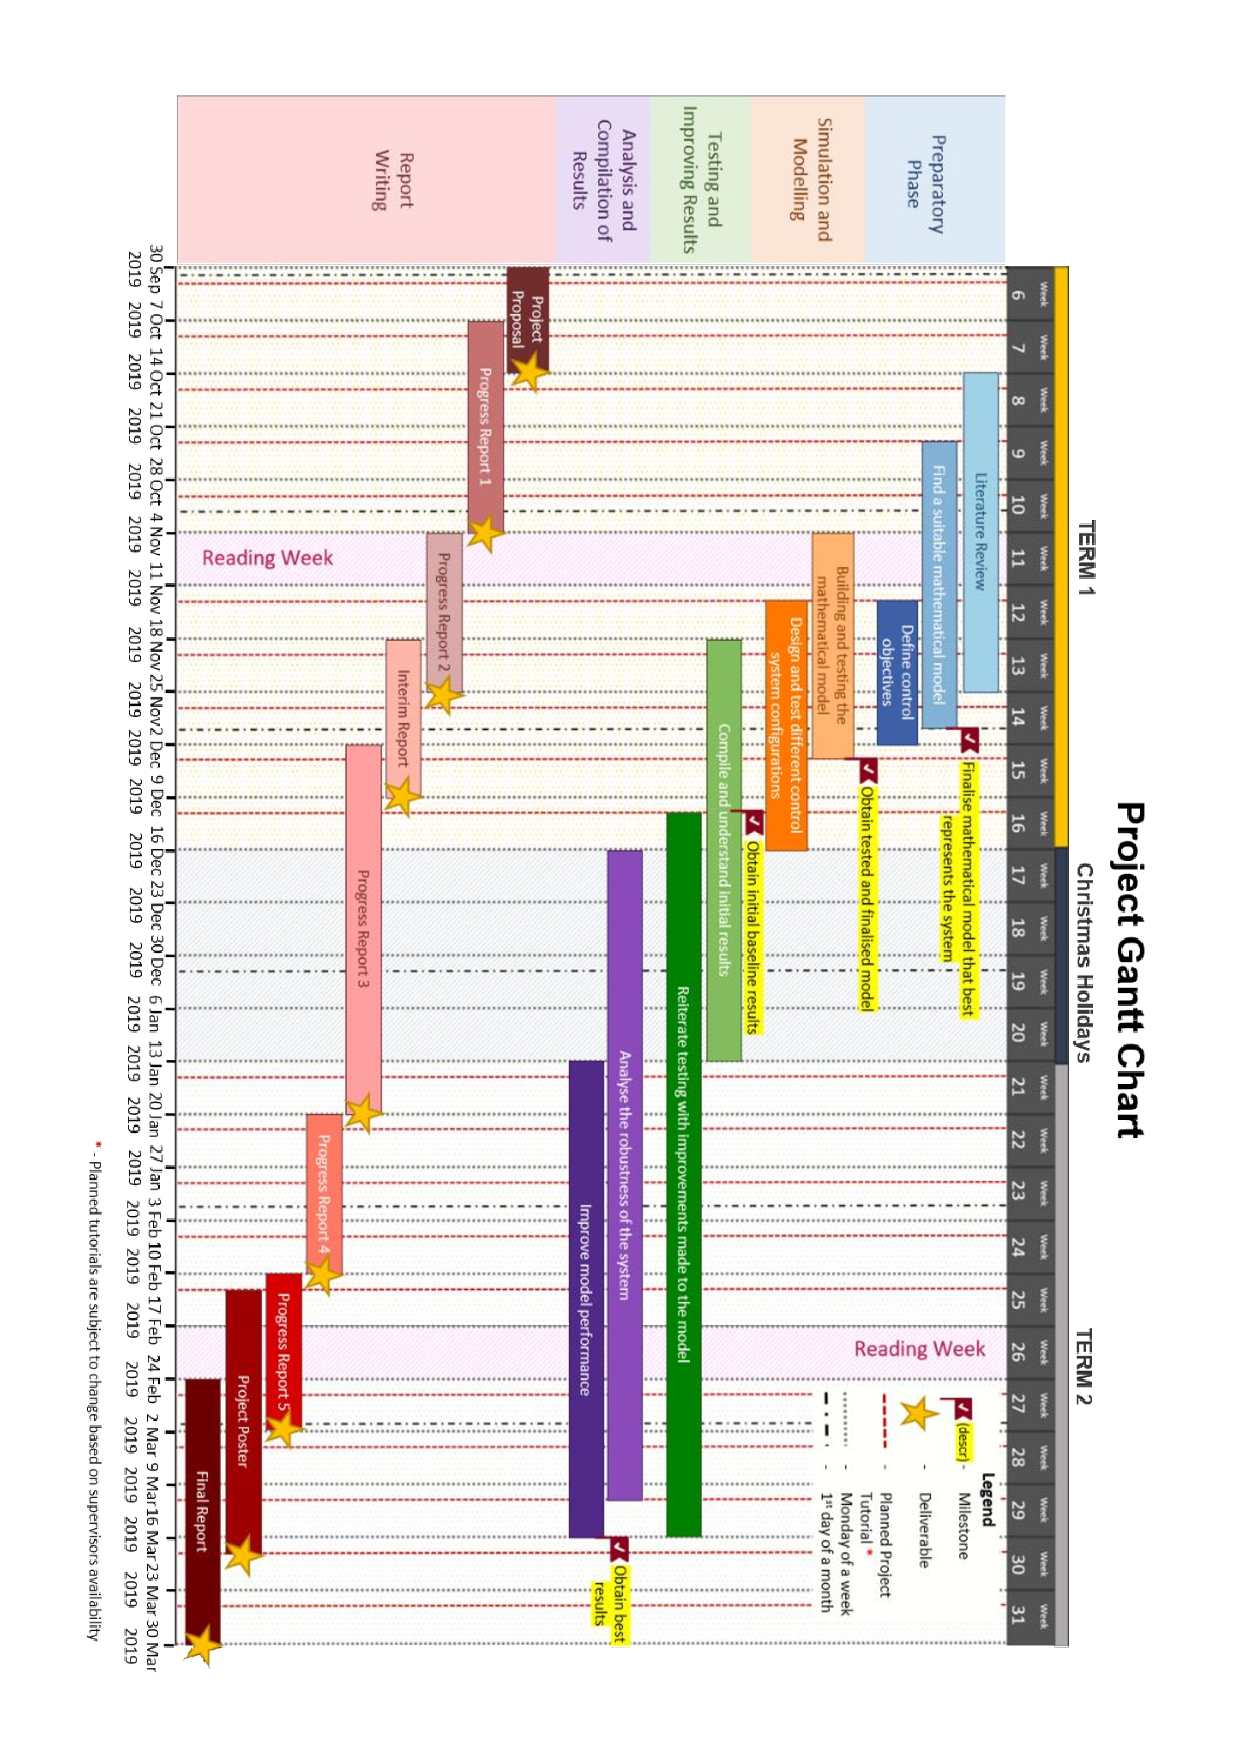
\includepdf[page=-]{files/Gantt Chart}
	\chapter{Risk Assessment}
	\label{appendix:b}
	The following hazards were identified through the risk assessment:
	\begin{itemize}
		\item Eyestrain
		\item Poor posture
		\item Repetitive movements involved with working on a computer
		\item Tripping over objects
		\item Poor lighting conditions
		\item Lone working
		\item Fire
		\item Contact with electricity
		\item General Welfare
	\end{itemize}
	The following pages includes a summary of the approved risk assessment generated using RiskNET.\\
	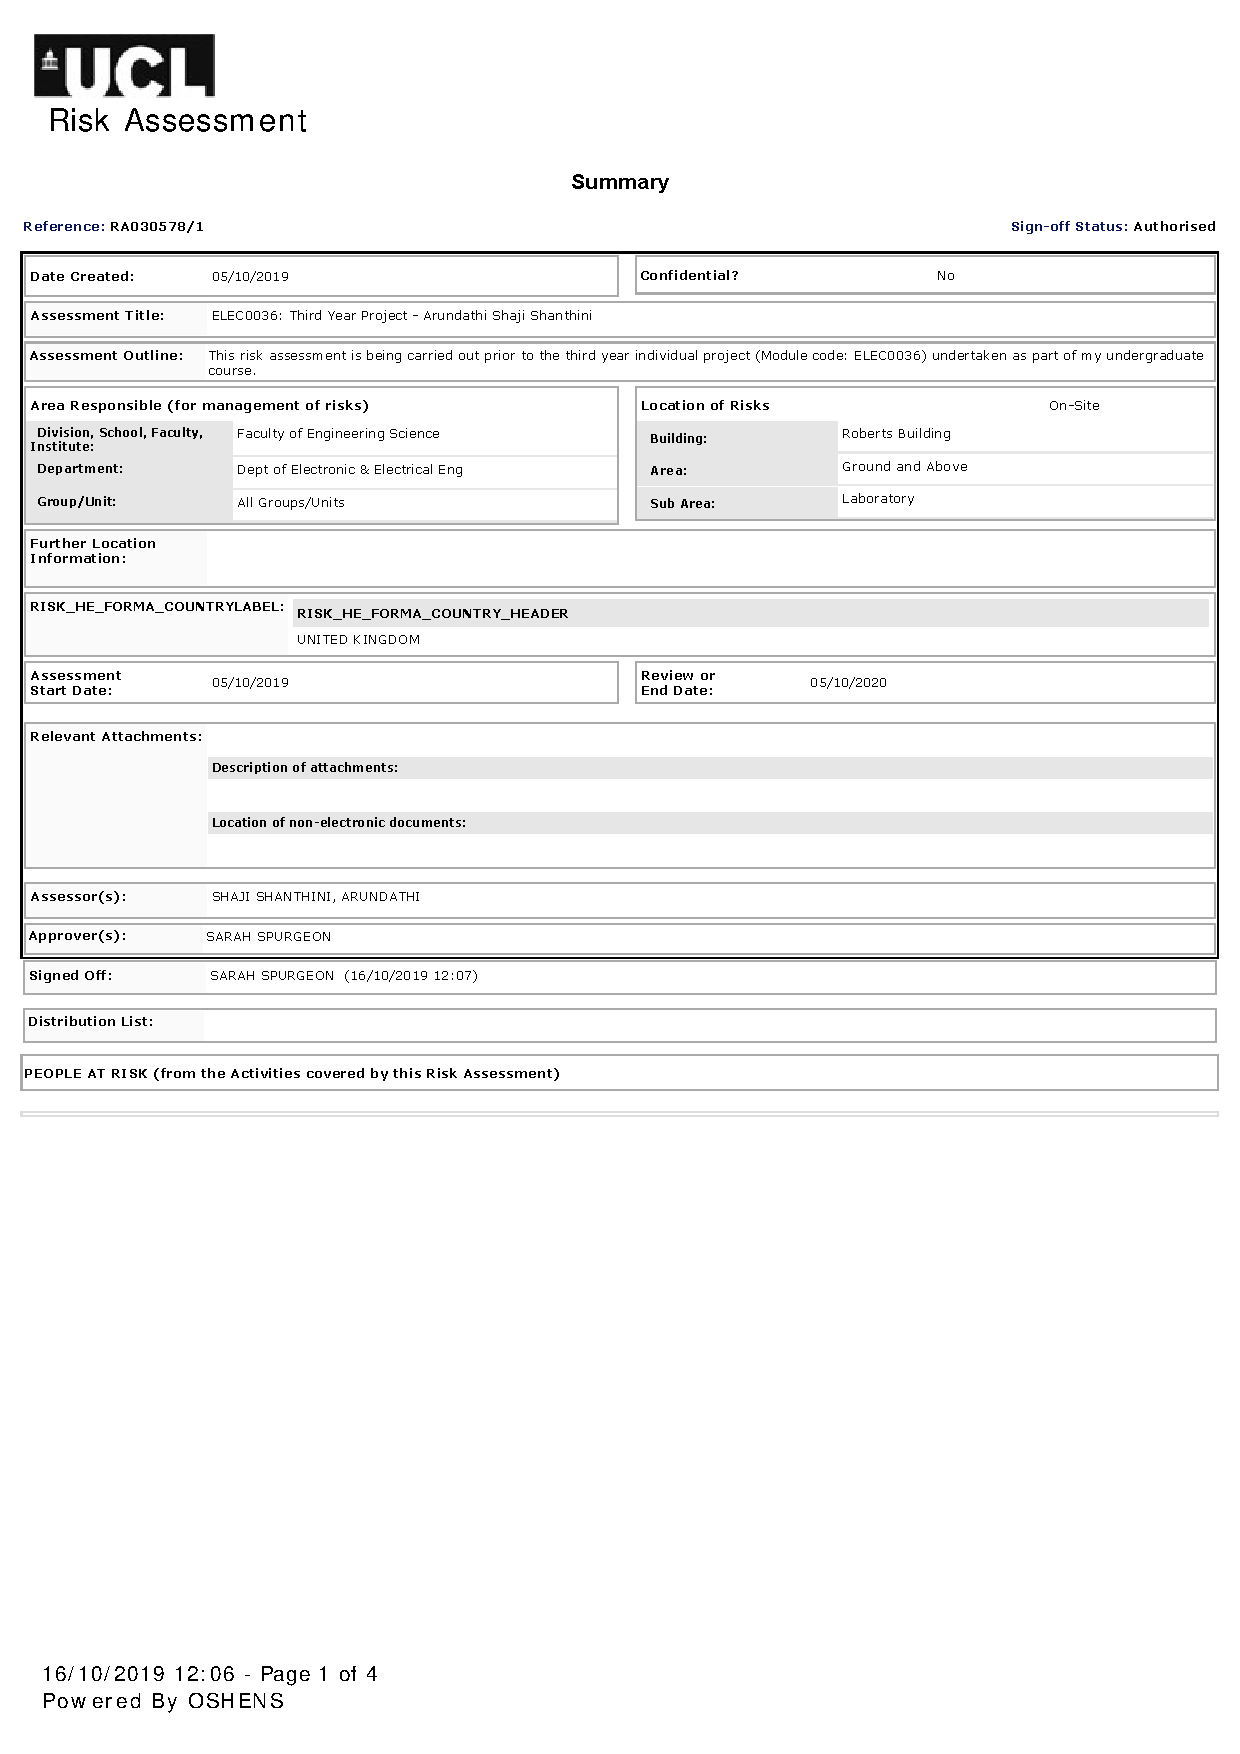
\includepdf[page=-]{files/Risk Assessment}
	\chapter{MATLAB Code}
	
\end{appendices}
%%%%%%%%%%%%%%%%%%%%%%%%%%%%%%%%%%%%%%

\bibliographystyle{IEEEtran}
\bibliography{references}

\end{document}